\documentclass[aspectratio=169]{beamer}
\usepackage[T1]{fontenc}
\usepackage[default]{sourcesanspro}
\usepackage{newtxsf}
\usepackage{hyperref}
\usepackage{latexsym,amsmath,xcolor,multicol,booktabs,calligra}
\usepackage{graphicx,pstricks,listings,stackengine}
\graphicspath{{./figures/}}
\usepackage{lipsum}
\usepackage{wrapfig}
\usepackage{url}
\usepackage{subcaption}
\usepackage{listings}
\usepackage{minted}
\setminted{fontsize=\footnotesize}
\usepackage{fontawesome5}

\usepackage{etoolbox}

\author{Yan Lin}
\title{AI Systems \& Infrastructure}
\subtitle{Module B.2: Container Fundamentals}
\institute{%
    \href{https://www.yanlincs.com}{www.yanlincs.com}
}
\date{September 1st, 2026}
\usepackage{AAU}
\AtBeginSubsection{}
\setbeamertemplate{navigation symbols}{}

\def\cmd#1{\texttt{\color{red}\footnotesize $\backslash$#1}}
\def\env#1{\texttt{\color{blue}\footnotesize #1}}
\definecolor{aauyellow}{RGB}{167, 131, 55}
\definecolor{aaublue}{RGB}{32, 26, 78}
\definecolor{aaured}{RGB}{152, 43, 28}
\definecolor{textgrey}{RGB}{60, 60, 60}

\setbeamercolor{normal text}{fg=textgrey}
\usebeamercolor[fg]{normal text}

\def\emphasis#1{{\color{aaured}\textbf{#1}}}
\renewcommand{\thefootnote}{}


\lstset{%
    basicstyle=\ttfamily\small,
    keywordstyle=\bfseries\color{deepblue},
    emphstyle=\ttfamily\color{deepred},
    stringstyle=\color{deepgreen},
    numbers=left,
    numberstyle=\small\color{halfgray},
    rulesepcolor=\color{red!20!green!20!blue!20},
    frame=shadowbox,
}

\begin{document}

\begin{frame}[plain,noframenumbering]
    \titlepage
    \vspace*{-0.6cm}
    \begin{figure}[htpb]
        \begin{center}
            
\includegraphics[keepaspectratio, scale=0.5]{aau-logo-left-uk}
        \end{center}
    \end{figure}
\end{frame}

\begin{frame}
\tableofcontents[sectionstyle=show,
subsectionstyle=show/shaded/hide,
subsubsectionstyle=show/shaded/hide]
\end{frame}


\section{The Problem}

\begin{frame}{It works on my machine}
\begin{minipage}[t]{0.6\textwidth}
    Our AI server from Module A.4 runs on your machine because you spent some time setting up Python, FastAPI, PyTorch, and possibly GPU drivers.

    \begin{itemize}
        \item A teammate would have to repeat the entire setup
        \item One missing system library or version conflict and things break
        \item Now imagine running the same server on a hundred machines in a data center
    \end{itemize}
\end{minipage}
\hfill
\begin{minipage}[t]{0.38\textwidth}
    \begin{figure}
        \begin{center}
            
\includegraphics[width=.9\textwidth]{programmer-reply}
        \end{center}
    \end{figure}
\end{minipage}
\end{frame}

\begin{frame}{Containers fix this}
    A \textbf{container} is a self-contained package of a program plus everything the program needs to run.
    The same package runs on any machine with a container runtime.

    \vspace{0.5em}
    Once our AI server is in a container, deploying to another machine becomes one or two commands.

    \vspace{0.5em}
    Containers are arguably the most important reason scaling AI deployment to thousands of computers is practical today.
\end{frame}


\section{What Is a Container}

\begin{frame}{The original shipping container}
Before \textbf{shipping containers} were standardized in the 1960s, freight was loaded onto ships piece by piece.
    Each shipment had its own size, shape, and packing, and dock workers had to figure out where everything went by hand.

    \begin{itemize}
        \item Loading a single ship could take days
        \item Goods often got damaged, lost, or stolen along the way
    \end{itemize}

    The fix is to agree on a standard box that any ship, train, or truck can carry, and pack everything into those boxes once at the source.

    \vspace{0.5em}
\textbf{Software containers} borrow both the idea and the name.
\end{frame}

\begin{frame}{Images vs containers}
    Two terms used interchangeably in everyday speech but with distinct meanings.

    \begin{block}{Container image}
        The package itself. A static, read-only blueprint of everything needed to run a program.
        Sits on disk and does nothing on its own.
        Like a recipe written on paper.
    \end{block}

    \begin{block}{Container}
        A running program created from an image.
        The runtime allocates CPU and memory, sets up an isolated environment, and runs the program inside it.
        Like the dish cooked from the recipe.
    \end{block}

    One image can be used to start many containers. Each starts in the same state and evolves independently.
\end{frame}

\begin{frame}{Container vs virtual machine}
\textbf{Virtual machines (VMs)} are the alternative approach to the same problem.

    \begin{figure}[htpb]
        \begin{center}
            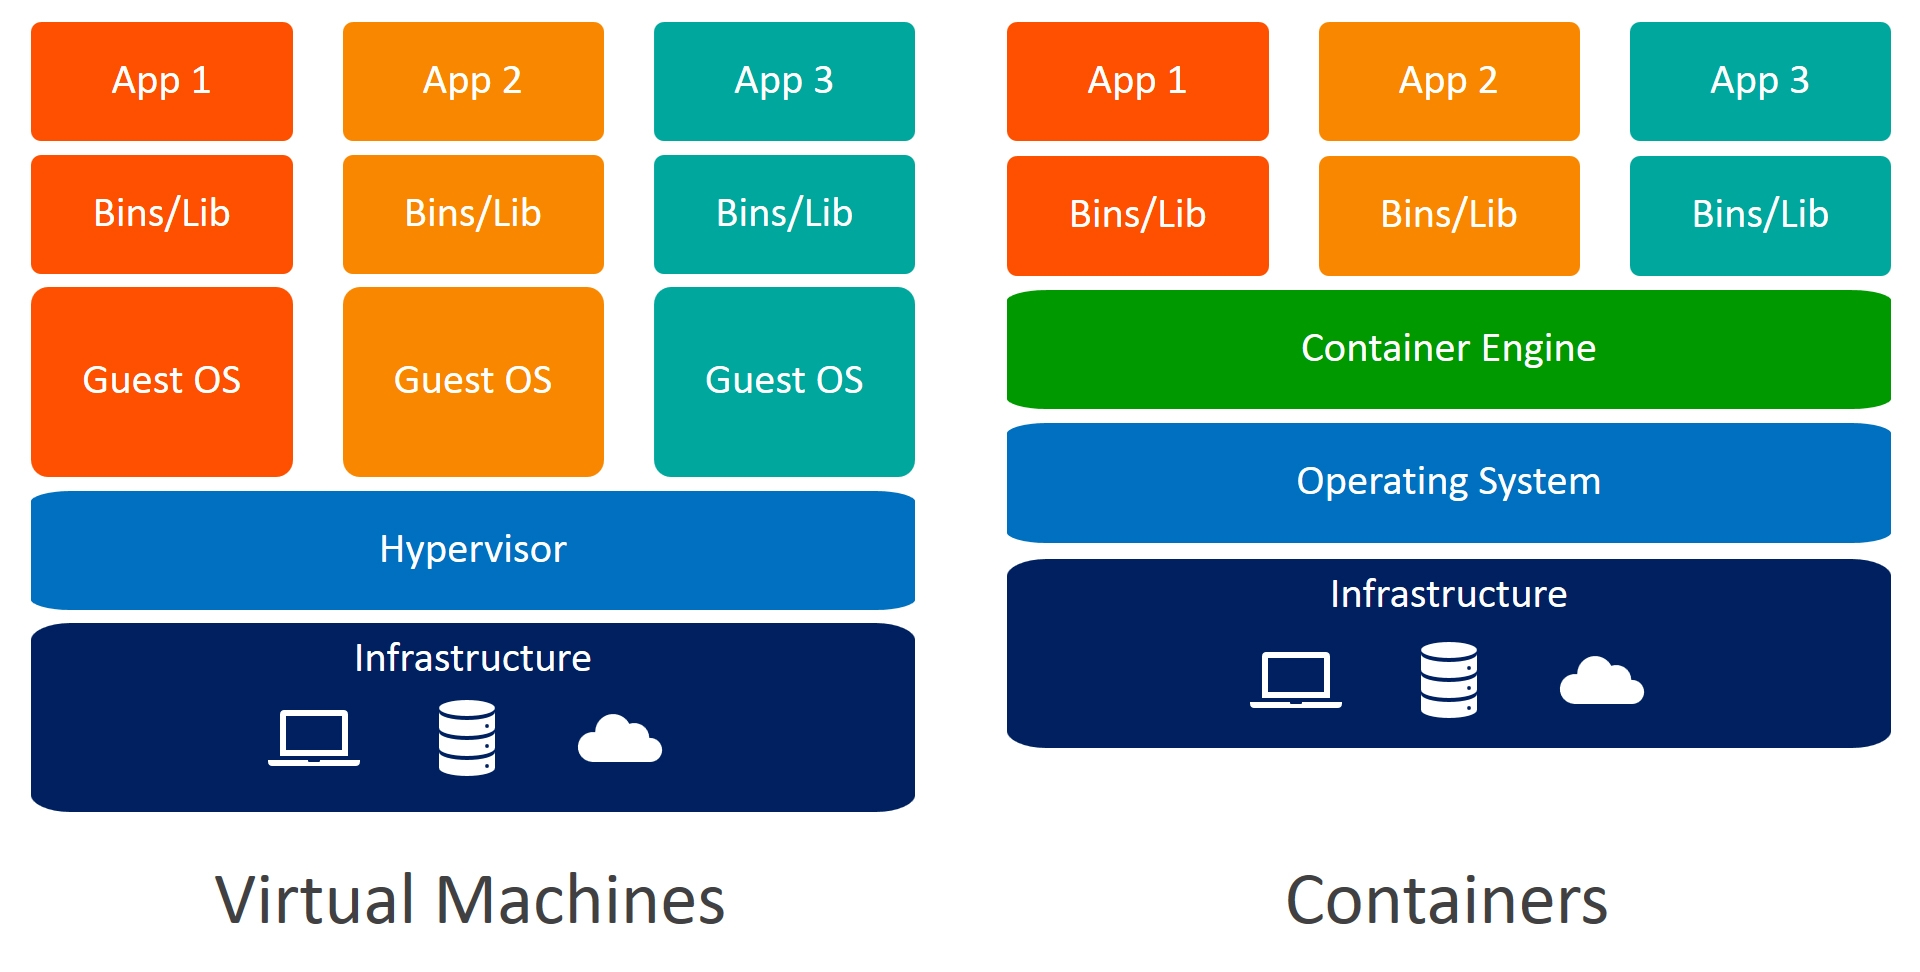
\includegraphics[width=0.6\textwidth]{vm_vs_container}
        \end{center}
    \end{figure}

Each virtual machine have its own kernel and operating system, while containers share the same host kernel.
Containers are light enough to start in seconds, at the cost of weaker isolation than a VM.
We come back to VMs in Module B.4.
\end{frame}

% TODO: The following two slides should be more intutiive and less technical, same with the corresponding content in the literature
\begin{frame}{Layered filesystems}
    The everything-the-program-needs inside an image is essentially a complete filesystem snapshot.
    Storing each image as one giant blob would be wasteful, since most images share a lot of common ground.

    \begin{figure}[htpb]
        \begin{center}
            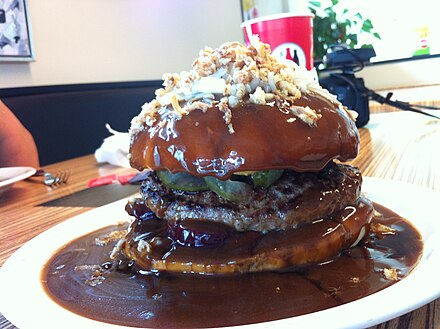
\includegraphics[width=0.32\textwidth]{danish-burger}
        \end{center}
    \end{figure}

    Think of burgers in a fast-food restaurant. The bottom bun and patty are shared.
    A cheeseburger adds cheese. A deluxe burger adds lettuce, tomato, and sauce.
\end{frame}

\begin{frame}[fragile]{Image as a stack of layers}
    A container image is built the same way, as a stack of read-only layers, each describing a small set of changes from the layer below.
    \begin{minted}{text}
4. Application code      <- /app/main.py copied in
3. Python packages       <- pip install ...
2. Python runtime        <- apt install python3
1. Debian base           <- /, /bin, /lib, etc.
    \end{minted}

    Each layer is a self-contained, content-addressed chunk on disk.
    Two images that share the same base only store that layer once.
    Pulling a new image only fetches the layers not already present.
\end{frame}

\begin{frame}{The writable layer}
    When a container starts from an image, the runtime adds one extra writable layer on top of the read-only stack.

    \begin{figure}[htpb]
        \begin{center}
            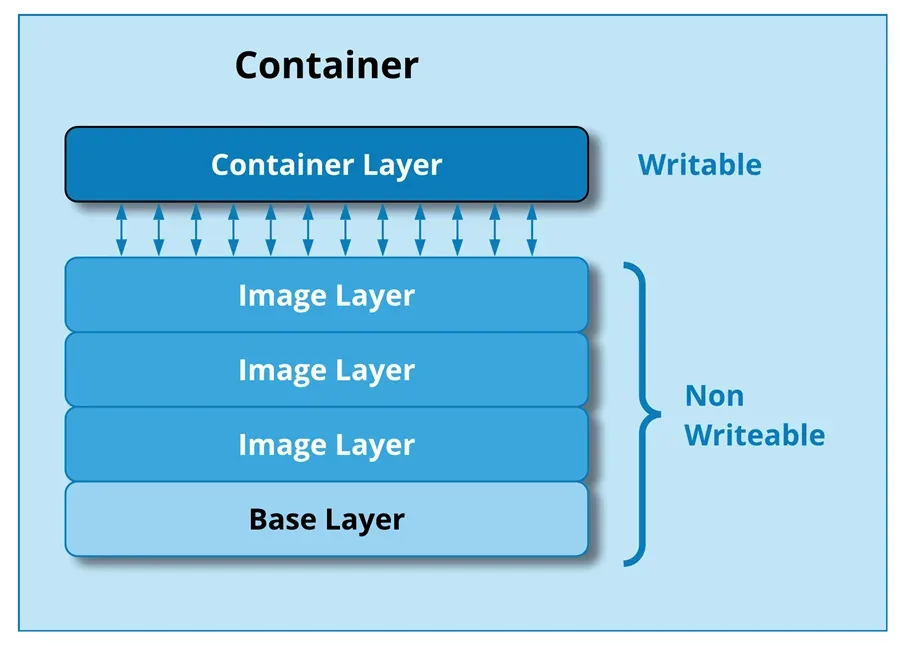
\includegraphics[width=0.4\textwidth]{container-layers}
        \end{center}
    \end{figure}

    Anything the running program writes, like temporary files, log lines, or cached data, ends up in that layer.
    When the container is removed, the writable layer is discarded.
\end{frame}

\begin{frame}{The OCI standard}
    We keep saying containers and runtimes as generic things, even though Docker is the household name.

    The reason is that the format and behavior of containers are governed by an open standard, not by any single vendor.

    \begin{block}{Open Container Initiative}
        An industry body that maintains the specification for what an image is and how a runtime should run one.
        Tools following OCI are interoperable.
    \end{block}

    \vspace{0.5em}
    Build an image with one tool, push it to a registry hosted by another, run it on a third. No conversion step in between.
\end{frame}


\section{The Docker Ecosystem}

\begin{frame}{Docker is not one program}
    Docker is the toolset that made containers mainstream, and it is still the most popular way to work with them.

    In practice, Docker is a collection of tools that work together.

    \begin{figure}[htpb]
        \begin{center}
            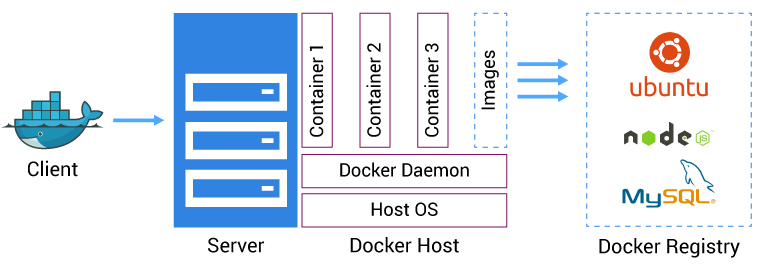
\includegraphics[width=0.8\textwidth]{docker-architecture}
        \end{center}
    \end{figure}
\end{frame}

\begin{frame}{Docker Engine and clients}
    \begin{block}{Docker Engine}
        The core runtime responsible for actually running containers on a machine.
        Pulls images, sets up namespaces and cgroups, starts and stops container processes.
        The server side is a long-running daemon (\texttt{dockerd}).
    \end{block}

    \begin{block}{Clients we will use}
        \begin{itemize}
\item \textbf{Docker CLI:} the \texttt{docker} command. Almost everything in this course goes through it
\item \textbf{Docker Desktop:} bundles the daemon, CLI, and a GUI into one installer
        \end{itemize}
    \end{block}
\end{frame}

\begin{frame}{Dockerfile and Docker Hub}
    \begin{block}{Dockerfile}
        Plain-text file describing how to build a container image.
        Each line is one instruction, roughly one layer per instruction.
        We will build our own in Module B.3.
    \end{block}

    \begin{block}{Docker Hub}
        Public registry where developers publish and download container images.
        Hosts both official images for popular software (Python, PostgreSQL, Nginx) and a large collection of community images.
    \end{block}
\end{frame}


\section{Using Off-the-Shelf Containers}

\begin{frame}[fragile]{Pull an image}
    \begin{minted}{bash}
docker pull python:3.13
    \end{minted}

    \begin{itemize}
        \item Argument is \texttt{<repository>:<tag>}
        \item Tag picks a version. Omitting defaults to \texttt{latest}
        \item Pinning a specific tag is safer than \texttt{latest}
        \item Smaller variants within one version number: \texttt{python:3.13-slim}, \texttt{python:3.13-alpine}
    \end{itemize}

    For images on a different registry:
    \begin{minted}{bash}
docker pull ghcr.io/some-user/some-image:v1
    \end{minted}

Use \texttt{docker images} to list all pulled images.
\end{frame}

\begin{frame}[fragile]{Run a container}
    \begin{minted}{bash}
docker run python:3.13
    \end{minted}
    Starts a container, runs the image's default command.

    \begin{minted}{bash}
docker run python:3.13 python -c "print('hello!')"
    \end{minted}
    Everything after the image name is the command to run inside.

    \begin{minted}{bash}
docker run -it python:3.13 bash         # interactive shell
docker run -d python:3.13 sleep 3600    # detached, in the background
    \end{minted}

    \texttt{-it} for interactive sessions, \texttt{-d} for long-running background services.
\end{frame}

\begin{frame}[fragile]{Managing containers}
    Each container gets an autogenerated ID and a silly two-word name like \texttt{eager\_tesla}.
    Choose your own with \texttt{--name}.

    \begin{minted}{bash}
docker run --name my-app -d python:3.13 sleep 3600

docker ps                # running containers
docker ps -a             # all, including stopped
docker stop my-app
docker start my-app
docker logs my-app
docker logs -f my-app    # follow live
docker exec -it my-app bash    # shell inside a running container
docker rm my-app         # remove a stopped container
    \end{minted}
\end{frame}

\begin{frame}{Talking to the outside}
    A container is isolated from our machine by design.
    Files written inside stay inside, ports are not reachable from outside, and it does not see any of the host's environment variables.

    \vspace{0.5em}
    It also means we need explicit ways to poke holes when we actually want the container to interact with the outside world.

    \vspace{0.5em}
    The three most common holes we open:
    \begin{itemize}
        \item Ports
        \item Files (volumes)
        \item Environment variables
    \end{itemize}
\end{frame}

\begin{frame}[fragile]{Port mapping}
    \begin{minted}{bash}
docker run -p 8000:8000 python:3.13 python -m http.server 8000
    \end{minted}

    \begin{itemize}
        \item Format is \texttt{-p <host\_port>:<container\_port>}
        \item Visit \texttt{http://127.0.0.1:8000} on the host to reach the container
    \end{itemize}

    The two ports do not have to match:
    \begin{minted}{bash}
docker run -p 3000:8000 python:3.13 python -m http.server 8000
    \end{minted}

    Server still listens on 8000 inside, but appears as 3000 on the host.
    Useful when several containers use the same internal port.
\end{frame}

\begin{frame}[fragile]{Volume mapping}
    \begin{minted}{bash}
docker run -v $(pwd):/app python:3.13 ls /app
    \end{minted}

    \begin{itemize}
        \item Format is \texttt{-v <host\_path>:<container\_path>}
        \item The current directory now appears as \texttt{/app} inside the container
        \item Changes on either side are visible to the other
    \end{itemize}

    \vspace{0.5em}
    Two uses:
    \begin{enumerate}
        \item Feed code or config into a container without baking it into the image
        \item Persist data (like a database file) past the container's lifetime
    \end{enumerate}
\end{frame}

\begin{frame}[fragile]{Environment variables}
    A container does not see the host's environment variables.
    Pass them in with \texttt{-e}.

    \begin{minted}{bash}
docker run -e OPENAI_API_KEY=sk-abc... python:3.13 \
    python -c "import os; print(os.getenv('OPENAI_API_KEY'))"
    \end{minted}

    For many variables, use a file:
    \begin{minted}{bash}
docker run --env-file .env python:3.13 \
    python -c "import os; print(dict(os.environ))"
    \end{minted}

    Same \texttt{.env} format as Module A.2, one \texttt{KEY=value} per line.
\end{frame}


\section{Exercise}

\begin{frame}{Run the A.2 client in a container}
    Run the chatbot script from Module A.2, but without installing Python or \texttt{requests} on the host.

    \begin{block}{Outline}
        \begin{enumerate}
            \item Open a terminal in the directory where your client program lives
            \item Run a container from a image with Python runtime, like \texttt{python:3.13}, with volume mapping to pass the program
            \item Inside the container, run \texttt{pip install requests} and run the client program
        \end{enumerate}
    \end{block}
\end{frame}

\begin{frame}{Extensions}
    \begin{enumerate}
        \item Replace the interactive install step with one \texttt{docker run} that installs the dependency and runs the script in a single line
        \item Run the same script through \texttt{python:3.13-alpine}. Notice the image is much smaller and everything still works
        \item Try \texttt{docker stats} on a running container, and \texttt{docker inspect} for the full configuration. Get a feel for what the daemon is actually managing
    \end{enumerate}

    \vspace{0.5em}
    By the end you have a feel for how containers run programs without any per-machine setup.
    Next module: build our own image instead of using someone else's.
\end{frame}


\begin{frame}{What you should walk away with}
    By the end of the exercise, you should be able to:
    \begin{enumerate}
        \item Understand how container works
        \item Familiar with the Docker ecosystem
        \item Run and manage a container with an off-the-shelf image
    \end{enumerate}

    \vspace{0.5em}
In the next module, we will learn how to build our own container image with everything needed to run our AI API server.
\end{frame}


\appendix

\begin{frame}[plain,noframenumbering]
\begin{center}
{\large Thank you!}
\vspace{1cm}
\\[0.5em]
{\small \faEnvelope\ \href{mailto:lyan@cs.aau.dk}{lyan@cs.aau.dk} \\
\faGlobe\ \href{https://www.yanlincs.com}{www.yanlincs.com}}
\end{center}
\end{frame}

\end{document}
